    %\subsubsection{VR integration and data visualization interface}
    %\label{subsubsec:VR_integration}
    %%Define the sections of the VR interface and how information is displayed
    %\input{Text/VR_integration}

    %% Figure of Real building next to VR
     \begin{figure}[t]
          \centering
          \includegraphics[width= \linewidth]{Images/RealvsVRBuildling}
          \caption{Comparison side by side of actual photography (left) of laboratory building used for experiment and virtual clone (right) modeled and simulated in VR for the Complexity analysis experiment in facade design.}
          \label{fig:RealVsVR}
        \end{figure}

        %% Figure of interior and exterior VR
     \begin{figure}[t]
          \centering
          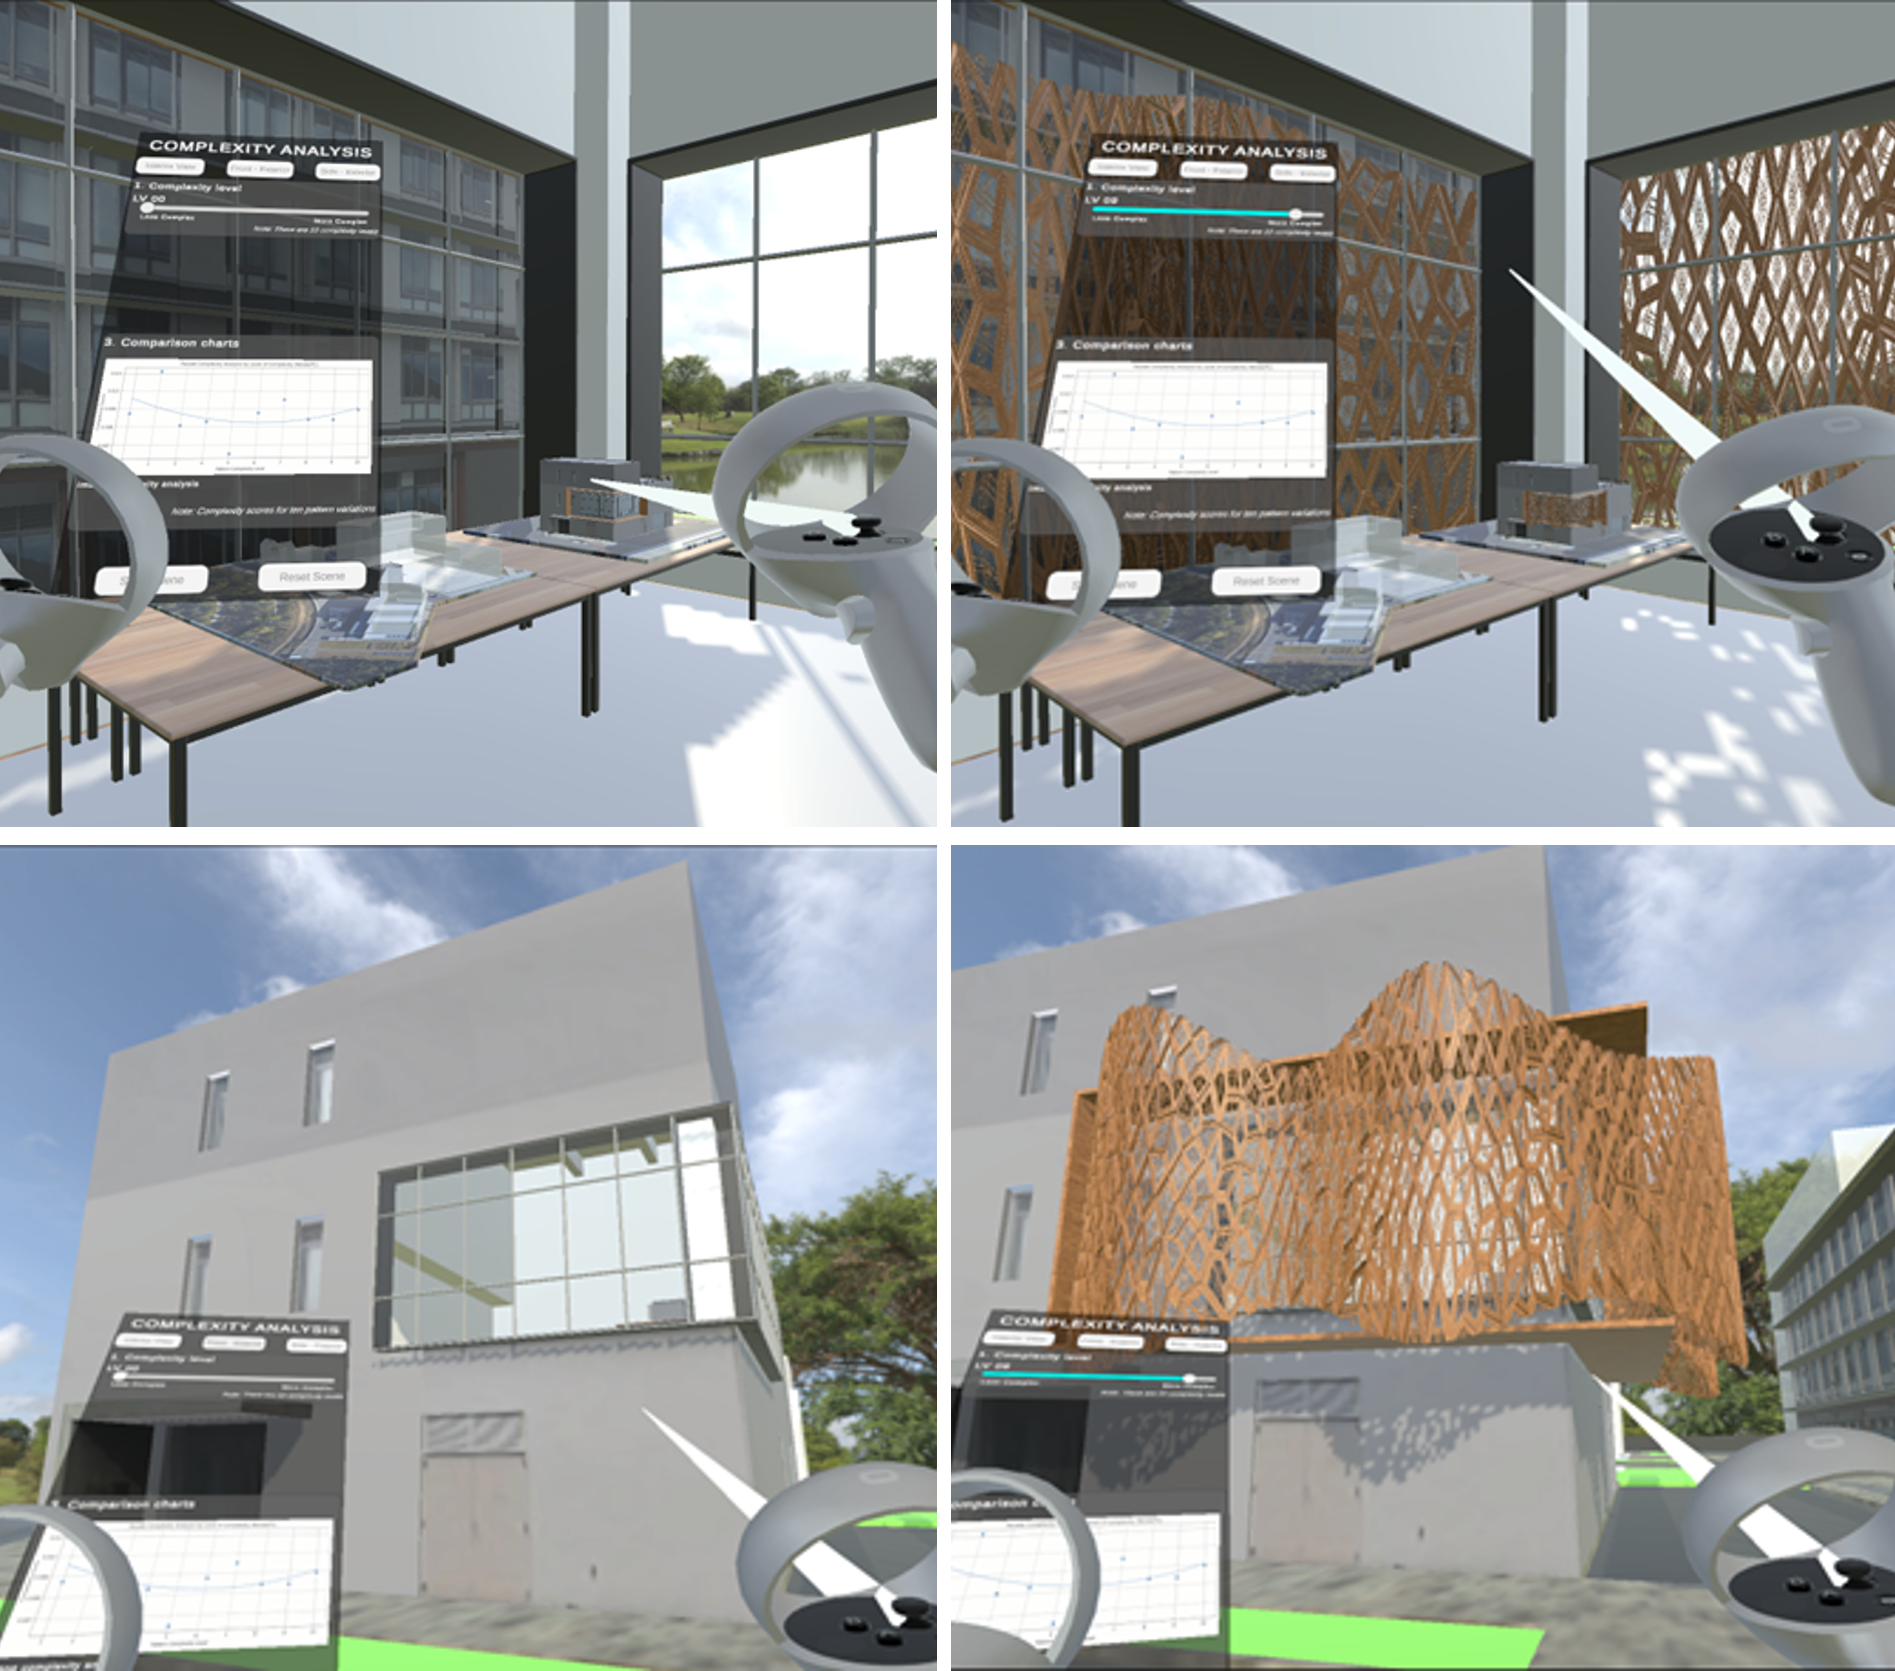
\includegraphics[width= \linewidth]{Images/VRInteriorExterior}
          \caption{VR simulation of interior and exterior of existing building at Kyushu University. (Left) Simulation of current building and (Right) simulation of Complex façade variation.}
          \label{fig:VRInteriorExterior}
        \end{figure}